

\section{IBM model 1}

\frame{
	\frametitle{MLE IBM 1}
	
	\begin{columns}
	\begin{column}{0.3\textwidth}
	\scalebox{0.8}{
    \begin{tikzpicture}
    % Define nodes
    \node[obs]						(f)		{$ f $};
    \node[right = of f]					(theta)		{\textcolor{red}{$\theta$}};
    %\node[const, above = of theta]					(alpha)		{$\alpha$};
    \node[latent, above = of f]		(a)		{$ a $};
    \node[cond, left = of f]		(e)		{$ e_0^{m} $};
    \node[cond, above = of e]		(m)		{$ m $};
    
    % Connect nodes
    \edge{e,a}{f};
    \edge{m}{a};
    \edge{theta}{f};
    %\edge{alpha}{theta};
    
    % add plates
    \plate {english-tables} {(theta)} {$ v_E $};
    \plate {source-sentence} {(f)(a)} {$ n $};
    \plate {corpus} {(source-sentence) (e) (m)} {$ S $};
    \end{tikzpicture}
    }
    \end{column}
    
	\begin{column}{0.7\textwidth}
	Global variables
    \begin{itemize}
	    \item For each English type \me, \\
	    we have a vector $\theta_\me$ of categorical parameters 
	    \begin{itemize} 
	    	\item $0< \theta_e < 1$
	    	\item $\sum_{f\in \mathcal F} \theta_{e,f} = 1$
	    \end{itemize}
	    and $P_{F|E}(f|e) = \Cat(F=f|\theta_e) = \theta_{e,f}$ 
    \end{itemize}
    \pause
    Local assignments
    \begin{itemize}
	    \item For each French word position $j$,
	    $$A_j \sim \mathcal U(0 \ldots m)$$
		$$F_j | e_{a_j} \sim \Cat(\theta_{e_{a_j}})$$
    \end{itemize}
	\end{column}	
	\end{columns}
	
	
}




\frame{
	\frametitle{Bayesian IBM 1}
	
	\begin{columns}
	\begin{column}{0.3\textwidth}
	\scalebox{0.8}{
    \begin{tikzpicture}
    % Define nodes
    \node[obs]						(f)		{$ f $};
    \node[latent, right = of f]					(theta)		{\textcolor{blue}{$\theta$}};
    \node[const, above = of theta]					(alpha)		{$\alpha$};
    \node[latent, above = of f]		(a)		{$ a $};
    \node[cond, left = of f]		(e)		{$ e_0^{m} $};
    \node[cond, above = of e]		(m)		{$ m $};
    
    % Connect nodes
    \edge{e,a}{f};
    \edge{m}{a};
    \edge{theta}{f};
    \edge{alpha}{theta};
    
    % add plates
    \plate {english-tables} {(theta)} {$ v_E $};
    \plate {source-sentence} {(f)(a)} {$ n $};
    \plate {corpus} {(source-sentence) (e) (m)} {$ S $};
    \end{tikzpicture}
    }
    \end{column}
    
	\begin{column}{0.7\textwidth}
	Global assignments
    \begin{itemize}
	    \item For each English type \me, \\
	    sample categorical parameters 
	    $$\theta_\me \sim \Dir(\alpha)$$
    \end{itemize}
    \pause
    Local assignments
    \begin{itemize}
	    \item For each French word position $j$,
	    $$A_j \sim \mathcal U(0 \ldots m)$$
		$$F_j | e_{a_j} \sim \Cat(\theta_{e_{a_j}})$$
    \end{itemize}
	\end{column}	
	\end{columns}
	
	
}


\frame{
	\frametitle{MLE vs Bayesian IBM1}
	
	\begin{columns}
	\begin{column}{0.5\textwidth}
	\begin{center}
    \scalebox{0.7}{
    \begin{tikzpicture}
    % Define nodes
    \node[obs]						(f)		{$ f $};
    \node[const, right = of f]					(theta)		{\alert{$\theta$}};
    \node[latent, above = of f]		(a)		{$ a $};
    \node[cond, left = of f]		(e)		{$ e_0^{m} $};
    \node[cond, above = of e]		(m)		{$ m $};
    
    % Connect nodes
    \edge{e,a}{f};
    \edge{m}{a};
    \edge{theta}{f};
    
    % add plates
    \plate {english-tables} {(theta)} {$ v_E $};
    \plate {source-sentence} {(f)(a)} {$ n $};
    \plate {corpus} {(source-sentence) (e) (m)} {$ S $};
    \end{tikzpicture}
    }
    
    \end{center}
    \end{column}
    
	\begin{column}{0.5\textwidth}
	\scalebox{0.7}{
    \begin{tikzpicture}
    % Define nodes
    \node[obs]						(f)		{$ f $};
    \node[latent, right = of f]					(theta)		{\textcolor{blue}{$\theta$}};
    \node[const, above = of theta]					(alpha)		{$\alpha$};
    \node[latent, above = of f]		(a)		{$ a $};
    \node[cond, left = of f]		(e)		{$ e_0^{m} $};
    \node[cond, above = of e]		(m)		{$ m $};
    
    % Connect nodes
    \edge{e,a}{f};
    \edge{m}{a};
    \edge{theta}{f};
    \edge{alpha}{theta};
    
    % add plates
    \plate {english-tables} {(theta)} {$v_E$}
    \plate {source-sentence} {(f)(a)} {$ n $};
    \plate {corpus} {(source-sentence) (e) (m)} {$ S $};
    \end{tikzpicture}
    }
    
	\end{column}	
	\end{columns}
	\begin{small}
	
	\pause
	
	Incomplete data likelihood
	\begin{equation}
		P(f_1^n|e_1^m, \alert{\theta_1^{v_E}}) = \prod_{j=1}^n \underbrace{\sum_{a_j=0}^m \overbrace{P(a_j|m) P(f_j|e_{a_j}, \alert{\theta_1^{v_E}})}^{P(f_j, a_j|e_1^m, \theta_1^{v_E})}}_{P(f_j|e_1^m, \theta_1^{v_E})}
	\end{equation}
	
	\pause
	
	Marginal likelihood (evidence)
	\begin{equation}
    \begin{aligned}
    	P(f_1^n|e_1^m, \alpha) &= \int p(\textcolor{blue}{\theta_1^{v_E}}|\alpha) P(f_1^n|e_1^m, \textcolor{blue}{\theta_1^{v_E}}) \mathrm{d}\textcolor{blue}{\theta_1^{v_E}} \\ \pause
			&= \int p(\textcolor{blue}{\theta_1^{v_E}}|\alpha) \prod_{j=1}^n \sum_{a_j=0}^m P(a_j|m) P(f_j|e_{a_j}, \textcolor{blue}{\theta}_{e_{a_j}}) \mathrm{d}\textcolor{blue}{\theta_1^{v_E}}
	\end{aligned}
	\end{equation}
	
	\end{small}
}



\frame{
	\frametitle{What is a Dirichlet distribution?}
	
	Dirichlet: $\theta_e \sim \Dir(\alpha)$ with $\alpha \in \mathbb R_{>0}^{v_F}$
	\begin{equation}
		\Dir(\theta_e | \alpha) = \frac{\Gamma(\sum_{f \in \mathcal F} \alpha_f)}{\prod_{f \in \mathcal F} \Gamma(\alpha_f)} \prod_{f \in \mathcal F} \theta_{e,f}^{\alpha_f-1}
	\end{equation}
	\begin{itemize}
		\item an exponential family distribution over probability vectors
		\item each outcome is a $v_F$-dimensional vector of probability values that sum to 1
		\item can be used as a prior over the parameters of a Categorical distribution
		\item that is, a Dirichlet sample can be used to specify a Categorical distribution\\
		e.g. $F|E=e \sim \Cat(\theta_e)$
	\end{itemize}
	
	Use this \beamerbutton{\href{https://github.com/uva-slpl/nlp2/blob/gh-pages/resources/notebooks/Dirichlet.ipynb}{notebook}} and this \beamerbutton{\href{https://en.wikipedia.org/wiki/Dirichlet_distribution}{wikipage}} to learn more 

}

\frame{
	\frametitle{Why a Dirichlet prior on parameters?}
	
	If we set the components of $\alpha$ to the same value, we get a symmetric Dirichlet, if that value is small the Dirichlet will prefer
	\begin{itemize}
		\item samples that are very peaked
		\item in other words, categorical distributions that concentrate on few outcomes
	\end{itemize}
	\pause
	~
	
	In MLE we choose one fixed set of parameters (via EM)\\
	
	\pause
	
	~
	
	In Bayesian modelling we average over all possible parameters
	\begin{itemize}
		\item where each parameter set is weighted by a prior belief
		\item we can use this as an opportunity to, for example, express our preferences towards ``peaked models''
	\end{itemize}
	
}

\frame{
	\frametitle{Contrast the Dirichlet samples}
	\begin{columns}
	\begin{column}{0.4\textwidth}
	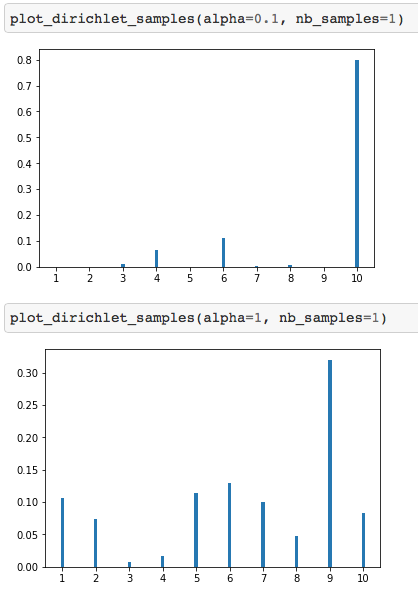
\includegraphics[scale=0.3]{dir-sample}
	\end{column}
	\begin{column}{0.6\textwidth}
	\begin{small}
	Top: sparse Dirichlet prior (small alpha)
	\begin{itemize}
		\item configurations that are this sparse will be roughly as likely
		\item less sparse configurations will be less likely
		\item ``the prior doesn't care where the tall bars are, as long as they are few''
	\end{itemize}
	
	\pause
	
	Take samples from the top Dirichlet to parameterise a Categorical distribution conditioning on English word ``dog''
	\begin{itemize}
		\item locations of the bars correspond to French words in the vocabulary
		\item the prior basically expresses the belief that whatever ``dog'' translates to, there shouldn't be many likely options available in French
	\end{itemize}
	\end{small}
	\end{column}
	\end{columns}
}

\frame{
	\frametitle{An alternative way to write the likelihood}
	
	We can write a likelihood based on Categorical events as follows
	\begin{small}
	\begin{equation}
	\begin{aligned}
		P(f_1^n, a_1^n|e_1^m, \theta_1^{v_E}) &= \prod_{j=1}^n \underbrace{P(a_j|m)}_{\frac{1}{m+1}}\underbrace{P(f_j|e_{a_j}, \theta_1^{v_E})}_{\theta_{f_j|e_{a_j}}} \\
		&= \frac{1}{(m+1)^n}\prod_{j=1}^n \theta_{f_j|e_{a_j}} 
		%&=\propto \prod_{j=1}^n \theta_{f_j|e_{a_j}}
	\end{aligned}
	\end{equation}
	\end{small}
	
	\pause
	an alternative way iterates over the vocabulary of pairs, rather than over the sentence
	\begin{small}
	\begin{equation}
	\begin{aligned}
		P(f_1^n, a_1^n|e_1^m, \theta_1^{v_E})
		&\propto \prod_{\me \in \mathcal E} \prod_{\mf \in \mathcal F} \theta_{\mf|\me}^{\#(\me \rightarrow \mf|f_1^n, a_1^n, e_1^m)}
	\end{aligned}
	\end{equation}
	\end{small}
	where $\#(\me \rightarrow \mf|f_1^n, a_1^n, e_1^m)$ counts how many times $\me$ and $\mf$ are aligned in the sentence pair $f_1^n, e_1^m$ given the alignments $a_1^n$
	
	
	\ack{I use $\theta_{e,f}$, $\theta_{e \rightarrow f}$, and $\theta_{f|e}$ interchangeably}
}

\frame{
	\frametitle{An alternative way to write the likelihood (cont)}
	
	The new form reveals similarities to the Dirichlet
	
	~
	
	Dirichlet prior
	\begin{small}
	\begin{equation}
	\begin{aligned}
		p(\theta_1^{v_E}|\alpha) &= \overbrace{\prod_{\me \in \mathcal E} \Dir(\theta_\me|\alpha)}^{\text{independent priors}} 
		 = \prod_{\me \in \mathcal E} \frac{\Gamma(\sum_{\mf \in \mathcal F} \alpha_\mf)}{\prod_{\mf \in \mathcal F} \Gamma(\alpha_\mf)} \prod_{\mf \in \mathcal F} \theta_{\mf|\me}^{\alpha_\mf-1}
	\end{aligned}
	\end{equation}
	\end{small}
	
	Multinomial (or Categorical likelihood)
	\begin{small}
	\begin{equation}
	\begin{aligned}
		P(f_1^n, a_1^n|e_1^m, \theta)
		&\propto \prod_{\me \in \mathcal E} \prod_{\mf \in \mathcal F} \theta_{\mf|\me}^{\#(\me \rightarrow \mf|f_1^n, a_1^n, e_1^m)}
	\end{aligned}
	\end{equation}
	\end{small}
	
	\pause
	
	Thus
	\begin{small}
	\begin{equation}
	\begin{aligned}
	p(\theta_1^{v_E},f_1^n,a_1^n|e_1^m, \alpha) &= p(\theta_1^{v_E}|\alpha) p(f_1^n,a_1^n|e_1^m, \theta_1^{v_E}) \\
	 &\propto \prod_{\me \in \mathcal E} \prod_{\mf \in \mathcal F} \underbrace{\theta_{\mf|\me}^{\alpha_\mf-1} \times \theta_{\mf|\me}^{\#(\me \rightarrow \mf|f_1^n, a_1^n, e_1^m)}}_{\pause \theta_{\mf|\me}^{\#(\me \rightarrow \mf|f_1^n, a_1^n, e_1^m) + \alpha_\mf - 1 }}
	\end{aligned}
	\end{equation}
	\end{small}
}

\frame{
	\frametitle{Bayesian IBM 1: Joint Distribution}
	
	Sentence pair: $(e_0^m, f_1^n)$
	\begin{footnotesize}
	\begin{equation*}
	\begin{aligned}
		p(f_1^n, a_1^n, \theta_1^{v_E}|e_0^m, \alpha) &= \overbrace{P(a_1^n|m)}^{\text{constant}} \underbrace{\prod_{\me \in \mathcal E}}_{\text{English types}} \overbrace{p(\theta_\me|\alpha)}^{\Dir \text{ prior}} \overbrace{\prod_{\me \in \mathcal E}\underbrace{\prod_{\mf \in \mathcal F}}_{\text{French types}} \theta_{\mf|\me}^{\#(\me \rightarrow \mf|f_1^n, a_1^n, e_1^m)}}^{\text{likelihood}} \\ \pause
		 &= P(a_1^n|m) \prod_\me \underbrace{\frac{\Gamma(\sum_\mf \alpha_\mf)}{\prod_\mf \Gamma(\alpha_\mf)} \prod_\mf \theta_{\mf|\me}^{\alpha_\mf - 1}}_{\text{Dirichlet}} \underbrace{\prod_\mf \theta_{\mf|\me}^{\#(\me \rightarrow \mf|f_1^n, a_1^n, e_1^m)}}_{\text{Categorical}} \\ \pause
		&\propto P(a_1^n|m) \prod_\me \prod_\mf \theta_{\mf|\me}^{\#(\me \rightarrow \mf|a_1^n) + \alpha_\mf - 1 }
		%&\quad{} \#(\me \rightarrow \mf|a_1^n) = \sum_{j=1}^n \mathds 1_\me(e_{a_j}) \times \mathds 1_\mf(f_j) \nonumber
	\end{aligned}
	\end{equation*}
	\end{footnotesize}
	
}

\frame{
	\frametitle{Bayesian IBM 1: Joint Distribution (II)}
	
	Sentence pair: $(e_0^m, f_1^n)$
	\begin{small}
	\begin{align}
		p(f_1^n, a_1^n, \theta_1^{v_E}|e_0^m, \alpha) &\propto P(a_1^n|m) \prod_\me \prod_\mf \theta_{\mf|\me}^{\#(\me \rightarrow \mf|f_1^n, a_1^n, e_1^m) + \alpha_\mf - 1 }
	\end{align}
	\end{small}
	
	Corpus: $(\mathbf e, \mathbf f)$
	\begin{small}
	\begin{equation}
	\begin{aligned}
		p(\mathbf f, \mathbf a, \theta_1^{v_E}|\mathbf e, \mathbf m, \alpha) 
		&\propto \prod_{(e_0^m, f_1^n, a_1^n)} P(a_1^n|m) \prod_\me \prod_\mf \theta_{\mf|\me}^{\#(\me \rightarrow \mf|f_1^n, a_1^n, e_1^m) + \alpha_\mf - 1 } \\
		&= P(\mathbf a|\mathbf m) \prod_\me \prod_\mf \theta_{\mf|\me}^{\#(\me \rightarrow \mf|\mathbf f, \mathbf a, \mathbf e) + \alpha_\mf - 1 }
	\end{aligned}
	\end{equation}
	\end{small}
	where I use boldface to indicate the collection 
}

\frame{
	\frametitle{Bayesian IBM 1: Inference}
	
	In Bayesian modelling {\bf there is no  optimisation}
	\begin{itemize}
		\item we {\bf do not} pick one model
		\item instead, we infer a posterior distribution over unknowns \\
		and reason using all models (or a representative sample)
	\end{itemize}
}

\frame{
	\frametitle{Bayesian IBM 1: Posterior}
	
	Intractable marginalisation

	\begin{align}
		p(\mathbf a, \theta_1^{v_E}|\mathbf e, \mathbf m, \mathbf f, \alpha) 
		&= \frac{p(\mathbf f, \mathbf a, \theta|\mathbf e, \mathbf m, \alpha)}{\int \sum_{\mathbf a'} p(\mathbf f, \mathbf a', \theta'|\mathbf e, \mathbf m, \alpha) \mathrm{d}\theta'}
	\end{align}
	
	\begin{itemize}
		\item $\theta_1^{v_E}$ are global variables: posterior depends on the entire corpus
		\item the summation goes over every possible alignment configuration for every possible parameter setting
	\end{itemize}

}


\frame{
	\frametitle{Bayesian IBM 1: Approximate inference}
	
	Traditionally, we would approach posterior inference with an approximate algorithm such as Markov chain Monte Carlo
	\begin{itemize}
		\item based on sampling from the posterior by sampling one variable at a time and forming a chain whose stationary distribution is the true posterior
	\end{itemize}
	
	~
	
	\pause
	
	MCMC is fully general, but can be hard to derive, and can be slow in practice
	
	\ack{\citet{Mermer+2011:BWA} introduce Bayesian IBM1 and derive a Gibbs sampler}
	
}

\frame{
	\frametitle{Variational inference}
	Optimise an auxiliary model to perform inference \pause
	\begin{itemize}
		\item postulate a family $\mathcal Q$ of tractable approximations $q(z)$ to true posterior $p(z|x)$\\ 
		where $z$ are latent variables and $x$ are observations \pause
		\item pick the member $q^*$ of $\mathcal Q$ that is closest to $p$\\
		measure closeness with $\KL$ divergence \beamerbutton{\href{https://en.wikipedia.org/wiki/Kullback–Leibler_divergence}{wikipage}} \pause
		\item use tractable $q^*$ instead of $p$ for inference and predictions
	\end{itemize}
	
	~ \pause
	
	Objective
	\begin{equation}
	\begin{aligned}
		q* &= \argmin_{q \in \mathcal Q} ~ \KL(q(z)||p(z|x)) \\ \pause
		 &= \argmin_{q \in \mathcal Q} ~ \mathbb E_{q(z)}\left[ \log \frac{q(z)}{p(z|x)}\right]
	\end{aligned}
	\end{equation}
}


\frame{
	\frametitle{Variational Inference - Objective}
	The original objective is intractable due to posterior
	\begin{equation*}
	\begin{aligned}
		q* &= \argmin_{q \in \mathcal Q} ~ \mathbb E_{q(z)}\left[ \log \frac{q(z)}{\alert{p(z|x)}}\right] \\ \pause
		&= \argmin_{q \in \mathcal Q} ~ \mathbb E_{q(z)}\left[ \log \frac{q(z)}{\frac{p(z, x)}{\alert{p(x)}}}\right] \\ \pause
		&= \argmin_{q \in \mathcal Q} ~ \mathbb E_{q(z)}\left[ \log \frac{q(z)}{p(z, x)}\right]  + \underbrace{ \alert{\log p(x)}}_{\text{constant}} \\ \pause
		&= \argmin_{q \in \mathcal Q} ~ - \mathbb E_{q(z)}\left[ \log \frac{p(z, x)}{q(z)}\right] \\ \pause
		&= \argmax_{q \in \mathcal Q} ~ \mathbb E_{q(z)}\left[ \log \frac{p(z, x)}{q(z)}\right] \\ \pause
		&= \argmax_{q \in \mathcal Q} ~ \mathbb E_{q(z)}\left[ \log p(z, x)\right] \underbrace{- \mathbb E_{q(z)}\left[ \log q(z) \right]}_{\mathbb H(q(z))}
	\end{aligned} 
	\end{equation*}
}

\frame{
	\frametitle{Evidence lowerbound (ELBO)}
	We've shown that minimising $\KL(q(z)||p(z|x))$ is equivalent to maximising a simpler objective
	\begin{equation*}
	\begin{aligned}
		q* &= \argmax_{q \in \mathcal Q} ~ \mathbb E_{q(z)}\left[ \log p(z, x)\right] + \mathbb H(q(z))
	\end{aligned} 
	\end{equation*}
	known as the evidence lowerbound \pause
	
	~
	
	For certain pairs of distributions in the exponential family, the quantities involved are both tractable
	\begin{itemize}
		\item e.g. the entropy of a Dirichlet variable is an analytical function of the parameter $\alpha$
		\item e.g. check \beamerbutton{\href{https://uva-slpl.github.io/nlp2/resources/papers/Schulz-BayesIBM1-tutorial.pdf}{this lecture script}} for analytical results for the first term
	\end{itemize}
	
	\ack{The name ELBO has to do with the fact that $\log p(x) \ge \text{ELBO}$}

}


\frame{
	\frametitle{How do we design $q$ for Bayesian IBM1?}
	
	Mean field assumption: make latent variables independent in $q$
	\begin{small}
	\begin{equation}
	\begin{aligned}
		q(a_1^n, \theta_1^{v_E}) &= q(\theta_1^{v_E}) \times Q(a_1^n) \\
		&= \prod_\me q(\theta_\me) \times \prod_{j=1}^n Q(a_j)
	\end{aligned}	\end{equation}
	\end{small}
	
	\pause

	Pick convenient parametric families
	\begin{small}
	\begin{equation}
	\begin{aligned}
		q(a_1^n, \theta_1^{v_E}|\phi, \lambda) &= \prod_\me q(\theta_\me|\lambda_\me) \times \prod_{j=1}^n Q(a_j|\phi_j) \\
		&= \prod_\me \Dir(\theta_\me|\lambda_\me) \times \prod_{j=1}^n \Cat(a_j|\phi_j)
	\end{aligned}
	\end{equation}
	\end{small}
	
	\pause
	Find optimum parameters under the ELBO
	\begin{itemize}
		\item one Dirichlet parameter vector $\lambda_\me$ per English type\\
		$\lambda_\me$ consists of $v_F$ strictly positive numbers 
		\item one Categorical parameter vector $\phi_j$ per alignment link\\
		$\phi_j$ consists of a probability vector over $m+1$ positions
	\end{itemize}
}

\frame{
	\frametitle{ELBO for Bayesian IBM1}
	Objective
	\begin{equation}
	\begin{aligned}
		(\hat{\lambda}, \hat{\phi}) &= \argmax_{\lambda, \phi}  \mathbb E_q[\log p(f_1^n, a_1^n, \theta_1^{v_E}|e_1^m, \alpha)] + \mathbb H(q)\\
		&= \argmax_{\lambda, \phi} \sum_{j=1}^m \mathbb E_q[\log P(a_j|m) P(f_j|e_{a_j}, \theta_1^{v_E}) - \log Q(a_j|\phi_j)] \\
		& ~~~~~~~~~~~ +\sum_\me \underbrace{\mathbb E_q[\log p(\theta_e|\alpha) - \log q(\theta_e|\lambda_e)]}_{-\KL(q(\theta_e|\lambda_e)||p(\theta_e|\alpha))}
	\end{aligned}
	\end{equation}

}

\begin{comment}
\frame{
	\frametitle{Bayesian IBM 1: Posterior (II)}
	
	Local variables
	\begin{align}
		P(a_j|e_0^m, f_j, \theta_1^{v_E}, \alpha) &= \frac{\overbrace{P(a_j|m)}^{\text{constant}}\overbrace{P(f_j,|e_{a_j}, \theta_1^{v_E}, \alpha)}^{\theta_{f_j|e_{a_j}}}}{\sum_{i=0}^m P(i|m)P(f_j,|e_{i}, \theta_1^{v_E}, \alpha)} 
	\end{align}
	\pause ~ thus $Q(a_j|\phi_j) = \Cat(a_j|\phi_j)$
	
	~
	
	\pause
	
	Global variables
	\begin{align}
		p(\theta_\me|\mathbf e, \mathbf f, \mathbf a, \alpha) &\propto \prod_{(e_0^m, f_1^n, a_1^n)} p(f_1^n, a_1^n, \theta_\me |e_0^m, \alpha) \\
		&= P(\mathbf a|\mathbf m) \prod_\me \prod_\mf \theta_{\mf|\me}^{\#(\me \rightarrow \mf|\mathbf a) + \alpha_\mf - 1 }
	\end{align}
	\pause ~ thus $q(\theta_e|\lambda_e) = \Dir(\lambda_e)$
}
\end{comment}


\frame{
	\frametitle{VB for IBM1}
	
	Optimal $Q(a_j|\phi_j)$ 
	\begin{align}
		\phi_{jk} &= \frac{\exp\left( \Psi\left(\lambda_{f_j|e_{k}}\right) - \Psi\left(\sum_\mf \lambda_{\mf|e_{k}}\right) \right)}{\sum_{i=0}^m \exp\left( \Psi\left(\lambda_{f_j|e_{i}}\right) - \Psi\left(\sum_\mf \lambda_{\mf|e_{i}}\right) \right)} 
	\end{align}
	~ where $\Psi(\cdot)$ is the \beamerbutton{\href{https://en.wikipedia.org/wiki/Digamma_function}{digamma function}}
	
	~
	
	Optimal $q(\theta_e|\lambda_e)$
	\begin{align}
		\lambda_{\mf|\me} = \alpha_\mf + \sum_{(e_0^m, f_1^n)} \sum_{j=1}^n \mathbb E_{Q(a_j|\phi_j)}[\#(\me \rightarrow \mf|f_j, a_j, e_1^m)]
	\end{align}
	
	\ack{For derivations check \beamerbutton{\href{https://github.com/philschulz/Reports/blob/master/VI/IBMVI/IBMVI.pdf}{Philip's notes}}}
}


\frame{
	\frametitle{Algorithmically}
	
	E-step as in MLE IBM1, \\
	~however, using $Q(a_j|\phi_j)$ instead of $P(a_j|e_0^m, f_j, \theta_1^{v_E})$ 
	\begin{itemize}
		\item equivalent to using $\theta \approx \hat{\theta}$ where
		\item $\hat{\theta}_{\mf|\me} = \exp\left( \Psi\left(\lambda_{\mf|\me}\right) - \Psi\left(\sum_{\mf'} \lambda_{\mf'|\me}\right) \right)$
	\end{itemize}
	
	\pause
	~
	
	M-step
	\begin{itemize}
		\item $\lambda_{\mf|\me} = \alpha_\mf + \mathbb E[\#(\me \rightarrow \mf)]$ \\
		where expected counts come from E-step
	\end{itemize}
	
}






